\documentclass{standalone}
\usepackage{tikz}
\usetikzlibrary{angles, quotes}

\begin{document}
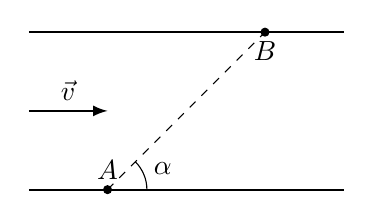
\begin{tikzpicture}   
	\coordinate (A) at (1,0);	
	\coordinate (B) at (3,2);
	\coordinate (C) at (4,0); 
	\draw [thick] (0,2) -- (4,2);
	\draw [thick] (0,0) -- (C);
	\draw [arrows={-latex}, thick] (0, 1) -- (1, 1) node [above, midway] {$\vec{v}$};
	\draw [dashed] (A) -- (B); 
	\draw [fill] (A) circle (0.05) node [above] {$A$};
	\draw [fill] (B) circle (0.05) node [below] {$B$};
	\pic [draw, -, angle eccentricity=1.5] {angle = C--A--B};
	\node [right=20pt, above = 2pt] at (A) {$\alpha$};
\end{tikzpicture}
\end{document}